%%%%%%%% ICML 2019 EXAMPLE LATEX SUBMISSION FILE %%%%%%%%%%%%%%%%%

\documentclass{article}

% Recommended, but optional, packages for figures and better typesetting:
\usepackage{microtype}
\usepackage{graphicx}
\usepackage{subfigure}
\usepackage{booktabs} % for professional tables

% hyperref makes hyperlinks in the resulting PDF.
% If your build breaks (sometimes temporarily if a hyperlink spans a page)
% please comment out the following usepackage line and replace
% \usepackage{icml2019} with \usepackage[nohyperref]{icml2019} above.
\usepackage{hyperref}

% Attempt to make hyperref and algorithmic work together better:
\newcommand{\theHalgorithm}{\arabic{algorithm}}

% Use the following line for the initial blind version submitted for review:
%\usepackage{icml2019}

% If accepted, instead use the following line for the camera-ready submission:
\usepackage[accepted]{icml2019}

% The \icmltitle you define below is probably too long as a header.
% Therefore, a short form for the running title is supplied here:
\icmltitlerunning{COSE474-2022F: Final Project Report}

\begin{document}

\twocolumn[
\icmltitle{COSE474-2021F: Final Project Proposal \\
           Trash Classification for Recycling with Object Detection}

% It is OKAY to include author information, even for blind
% submissions: the style file will automatically remove it for you
% unless you've provided the [accepted] option to the icml2019
% package.

% List of affiliations: The first argument should be a (short)
% identifier you will use later to specify author affiliations
% Academic affiliations should list Department, University, City, Region, Country
% Industry affiliations should list Company, City, Region, Country

% You can specify symbols, otherwise they are numbered in order.
% Ideally, you should not use this facility. Affiliations will be numbered
% in order of appearance and this is the preferred way.
\icmlsetsymbol{equal}{*}

\begin{icmlauthorlist}
{Yusung Min}
\end{icmlauthorlist}

%\icmlaffiliation{ku}{Department of Computer Science \& Engineering, Korea University, Seoul, Korea}


%\icmlcorrespondingauthor{the}{myemail@korea.ac.kr}
%\icmlcorrespondingauthor{Eee Pppp}{ep@eden.co.uk}

% You may provide any keywords that you
% find helpful for describing your paper; these are used to populate
% the "keywords" metadata in the PDF but will not be shown in the document
\icmlkeywords{Machine Learning, ICML}

\vskip 0.3in
]

% this must go after the closing bracket ] following \twocolumn[ ...

% This command actually creates the footnote in the first column
% listing the affiliations and the copyright notice.
% The command takes one argument, which is text to display at the start of the footnote.
% The \icmlEqualContribution command is standard text for equal contribution.
% Remove it (just {}) if you do not need this facility.

%\printAffiliationsAndNotice{}  % leave blank if no need to mention equal contribution
%\printAffiliationsAndNotice{\icmlEqualContribution} % otherwise use the standard text.

\begin{abstract}
{The goal of this project is to create a garbage classification model for recycling separation using object detection technology, and eventually to detect garbage in photos taken through smartphone cameras and tell them how the garbage should be classified. I got the dataset which has six classes from roboflow. For object detection model, and I used YOLOv5 Model for object detection.}
\end{abstract}

\section{Introduction}
{Currently, garbage emissions are increasing in our society. The government is trying several methods to encourage recycling and improving the recycling system. However, it is not easy to solve because people have to classify garbage themselves. The biggest reason for not properly separating trash is that they do not know how to do well. Therefore, We are going to try to develop a trash classification model. For developing model, object detection is necessarily required to distinguish garbage in image. After that, image classification should be learned to distribute which material these detected objects are.} \\

\section{Problem definition \& challenges}
{For sustainable society, recycling trash is inevitable for human being. According to Ministry of Environment of Republic of Korea, each Korean citizen produces 55 tons of garbage over his lifetime. Although there are only 5 years left until current landfill is available, in capital area, it is hard to find new site for creating landfill. Also garbage made of materials such as plastic do not rot easily and generate environmental hormones during incineration. For solving those problems, separating trash for recycling is necessary.
}\\
\section{Related Works}
{Object Detection. Object detection is still one of the fields actively studied. Since it is a difficult task to satisfy two tasks, object localization and classification, various models have been proposed so far. For example, various models have been developed, ranging from Faster-RCNN\cite{rcnn}, which built a two-stage detection pipeline using Region Proposal Network (RPN) and pre-trained convolution network in Fig. 1, to YOLO\cite{yolo}, which is based on single-stage model. Among these detection models, we plan to construct a garbage object detection model by fine-tuning YOLOv5(Zhu et al., 2021), a one-stage model using CNN backbone in Fig. 2.
}\\
\begin{figure}
\centering
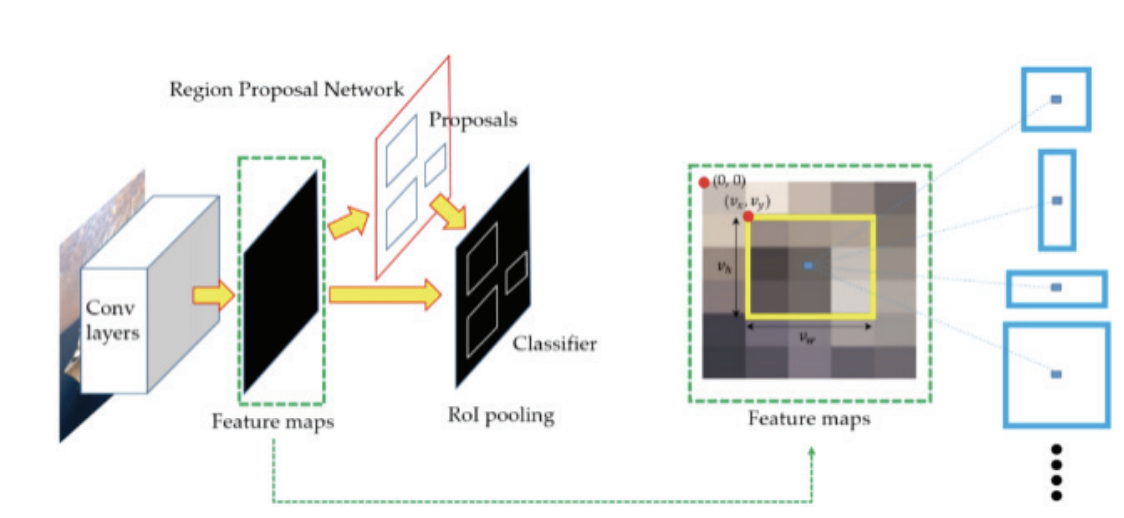
\includegraphics[width=7cm]{Final_Project/image/f-rcnn.png}
\caption{Structure of Faster-RCNN}
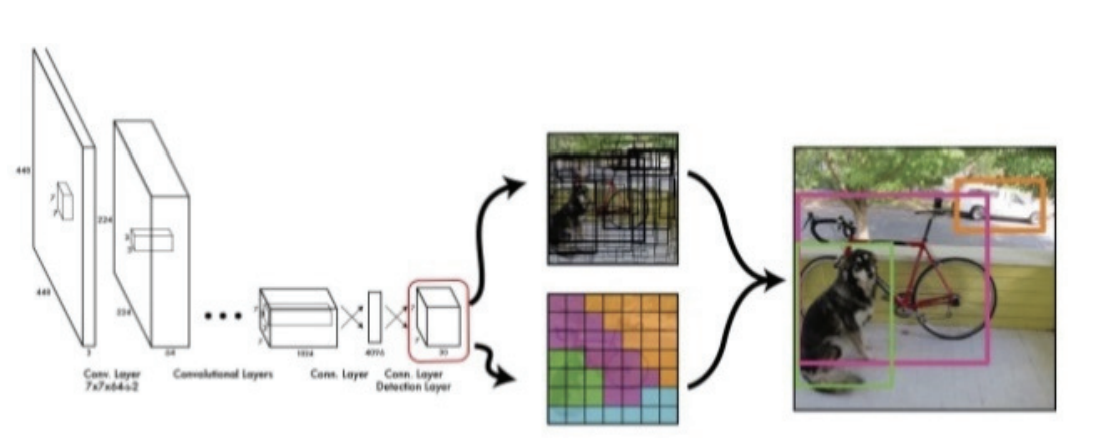
\includegraphics[width=7cm]{Final_Project/image/yolo structure.png}
\caption{Structure of YOLO }
\end{figure}
\section{Methods}
\subsection{Main challenges}
{In order to create a model that can help recycle, it is necessary to match the class label of what kind it is, beyond simply being able to determine whether it is trash or not. In addition, for using this model in practice, even if there are multiple objects in one picture, each class must be matched, also test speed must be fast. In addition, AI Model API Server is necessary to interact with the model and users.}\\
{To solve the above problem, the YOLO model was selected. Although I considered between YOLO and Faster-Rcnn, YOLO operates faster as a single stage and does not fall far behind in terms of performance, compared to Faster-Rcnn which is a multi-stage-based model.\cite{compare} Then I used Flask uses python to create API Server because model is created by python. Finally,  I used React Native to create simple application to show the model works.
}\\
\subsection{Architecture}
\begin{equation}\label{eq1}
GIoU(A,B) = IoU(A,B) - \frac{|C|-|A\cup B|}{|C|} 
\end{equation}
\\
\begin{equation}\label{eq2}
    {Loss_{GIoU}}^{} = 1 - GIoU(A,B) 
\end{equation}\\
{In this project, YOLOv5s Model was selected where C is the smallest box which is containing A and B. GIoU overcomes the distributed situation of A and B in IoU. Furthermore it has the same scale-invariance as IoU.
GIoU is less than or equal to IoU, so it can be considered the lower bound of IoU. GIoU not only pays attention to the overlapping area but also to other non-overlapping areas, which can be better to reflect the degree of overlap between of them. When the two boxes have no overlapping area, GIoU is a number that varies in the range of [−1, 0], and there is a gradient, so optimization can be performed. The optimization direction gradually narrows the distance between the two boxes.\cite{wangyolo}

\begin{figure}[!htb]
    \centering
    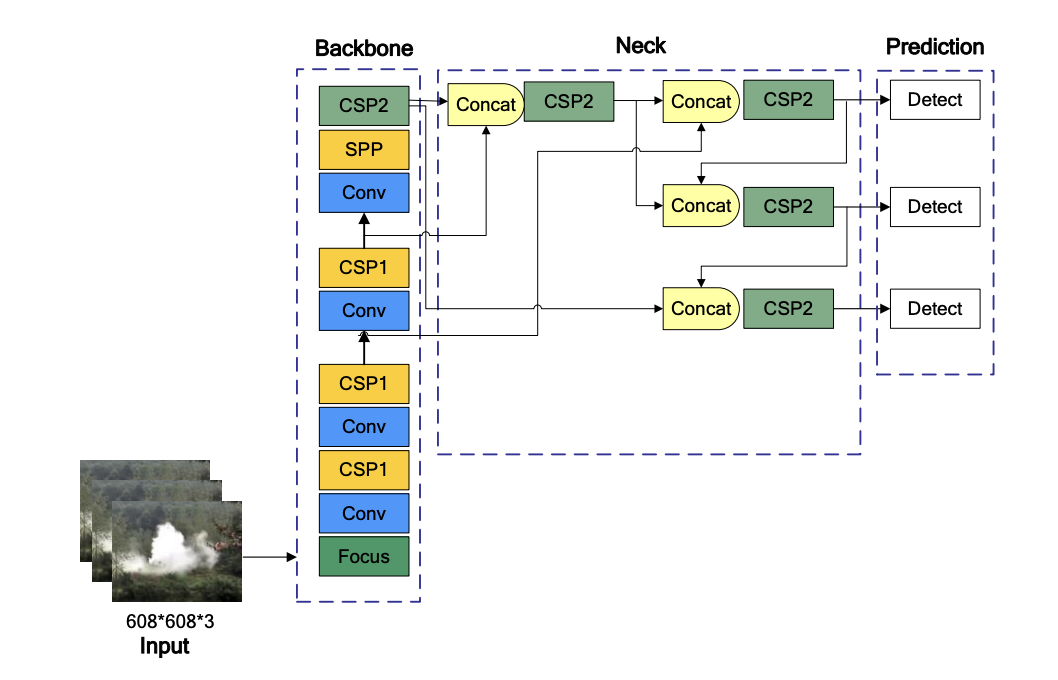
\includegraphics[width=7cm]{Final_Project/image/yolov5 network structure.png}
    \caption{YOLOv5 Network Structure}
    \label{fig:my_label}
\end{figure}
{At Fig. 3, it describes Network Structure of YOLOv5 model. The network consists of three main parts: backbone, neck, and output. Backbone part focuses on extracting feature information from input images, neck part fuses the extracted feature information and generates three scales of feature maps, and the output part detects the objects from these generated feature maps.\cite{yolo}}
\section{Experiments}
\subsection{Project Environment}
{For the smooth progress of the project, the project was carried out using the cloud-based collaboration service provided by Google.}
\\
\subsection{Datasets}
{The data acquisition process is simple. We found a dataset
includes garbage images from Roboflow.\cite{garbage-classification-3_dataset} The dataset contains
images of 7 types of trash, types are cardboard, glass, metal, paper, plastic, cloth and biodegradable. It contains total 10,464 images. However, we felt the need to increase the number of images to improve the performance of the model. Therefore, about 20\% of images were added through data augmentation. For For proper work for data augmentation, as shown in Fig. 4, we reversed the random training images from left to right. In addition, it is also necessary to do operation to reverse boundary box's coordinate values. Furthermore, we tried to improve the performance of the model by resizing the image to 320x320. Finally, 70\% of images are used for training, 20\% for validation and 10\% are used for testing. }\\
\begin{figure}[!htb]
    \centering
    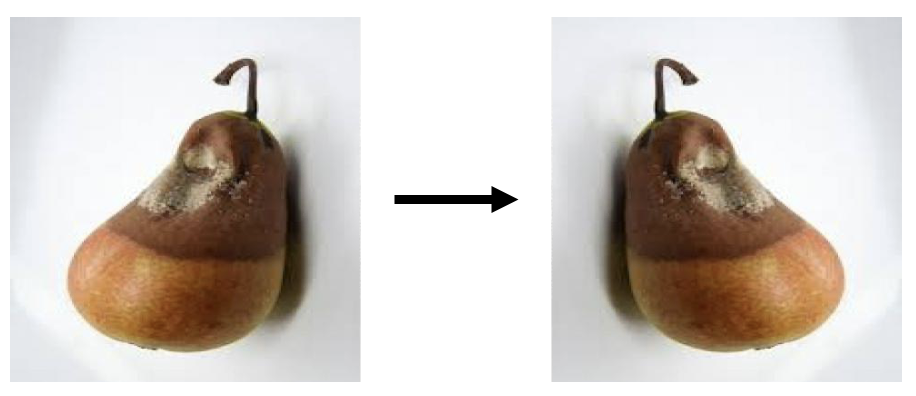
\includegraphics[width=7cm]{Final_Project/image/reversed data.png}
    \caption{Data Augmentation}
    \label{fig:my_label}
\end{figure}
\subsection{Implementations}
{The first step in the process of this project is preprocessing data. For this, we resized images 320 x 320 size and augmented data, and also divided data for training, validation, and test. Next, we constructed a model. We used YOLOv5s Model and trained model with above train dataset.
After that, we got best fit model and validated with validation dataset. At Fig. 5, it shows about the model's performance of YOLO. Mean average precision called MAP is used to evaluate model. If it is low, it means that the performance is not good, and if it is high, it means that it is good. When confidence is adjusted to 0.5, MAP is measured high. And the value was improved by 0.5 compared to when the data was not augmented.
 }\\
\begin{figure}[!htb]
    \centering
    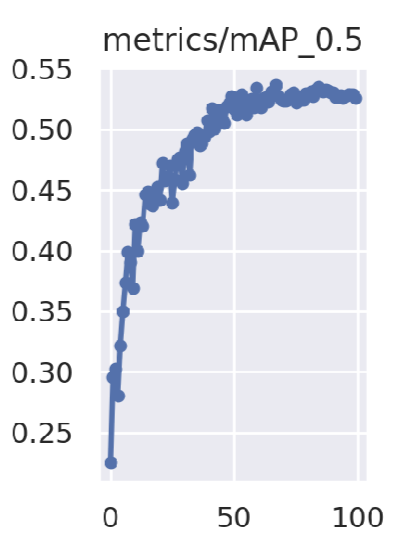
\includegraphics[width=4cm,height=5cm]{Final_Project/image/map.png}
    \caption{MAP of Model}
\end{figure}\\

\subsection{Compared with SOTA}
{DETReg which is about Class-agnostic Object Detection with Multi-modal Transformer has 84.16\% of MAP.\cite{maaz2022class} By contrast, my model has only about 53.19\% of MAP. But this model is faster than DETReg to object detect in real time, so our model is more appropriate for our project.}

\subsection{Application}
{Our project's final goal is to use this model in practice, so we developed simple client with React Native. And then, we construct API server for our model by Flask. Fig. 6 is result of our project. We actually took a photo a bottle of yogurt made of plastic and a torn box of snack. This model also detected real objects well. The torn box was recognized as two objects, but in fact, it is almost half torn, so it is not judged that there is a performance problem. }
\begin{figure}[!htb]
    \centering
    \includegraphics[width=7cm,height=6cm]{Final_Project/image/test1.jpeg}
    \caption{Result of applying to device}
    \label{fig:my_label}
\end{figure}\\

\section{Discussion \& Future Direction}
This project was quite successful, but not perfect. The advantage of YOLO model is that object detection can be performed with real time, but it could not be performed with real time by loading the model through the API server, not putting it directly into the device. Therefore, in order to take advantage of real time, it seems necessary to put it directly into the device using a smaller model. Another problem is that it does not have a certain probability for all classes and detects only specific classes well.  However, since there is not much difference, this will need to be addressed through data supplementation.
\begin{figure}[!htb]
    \centering
    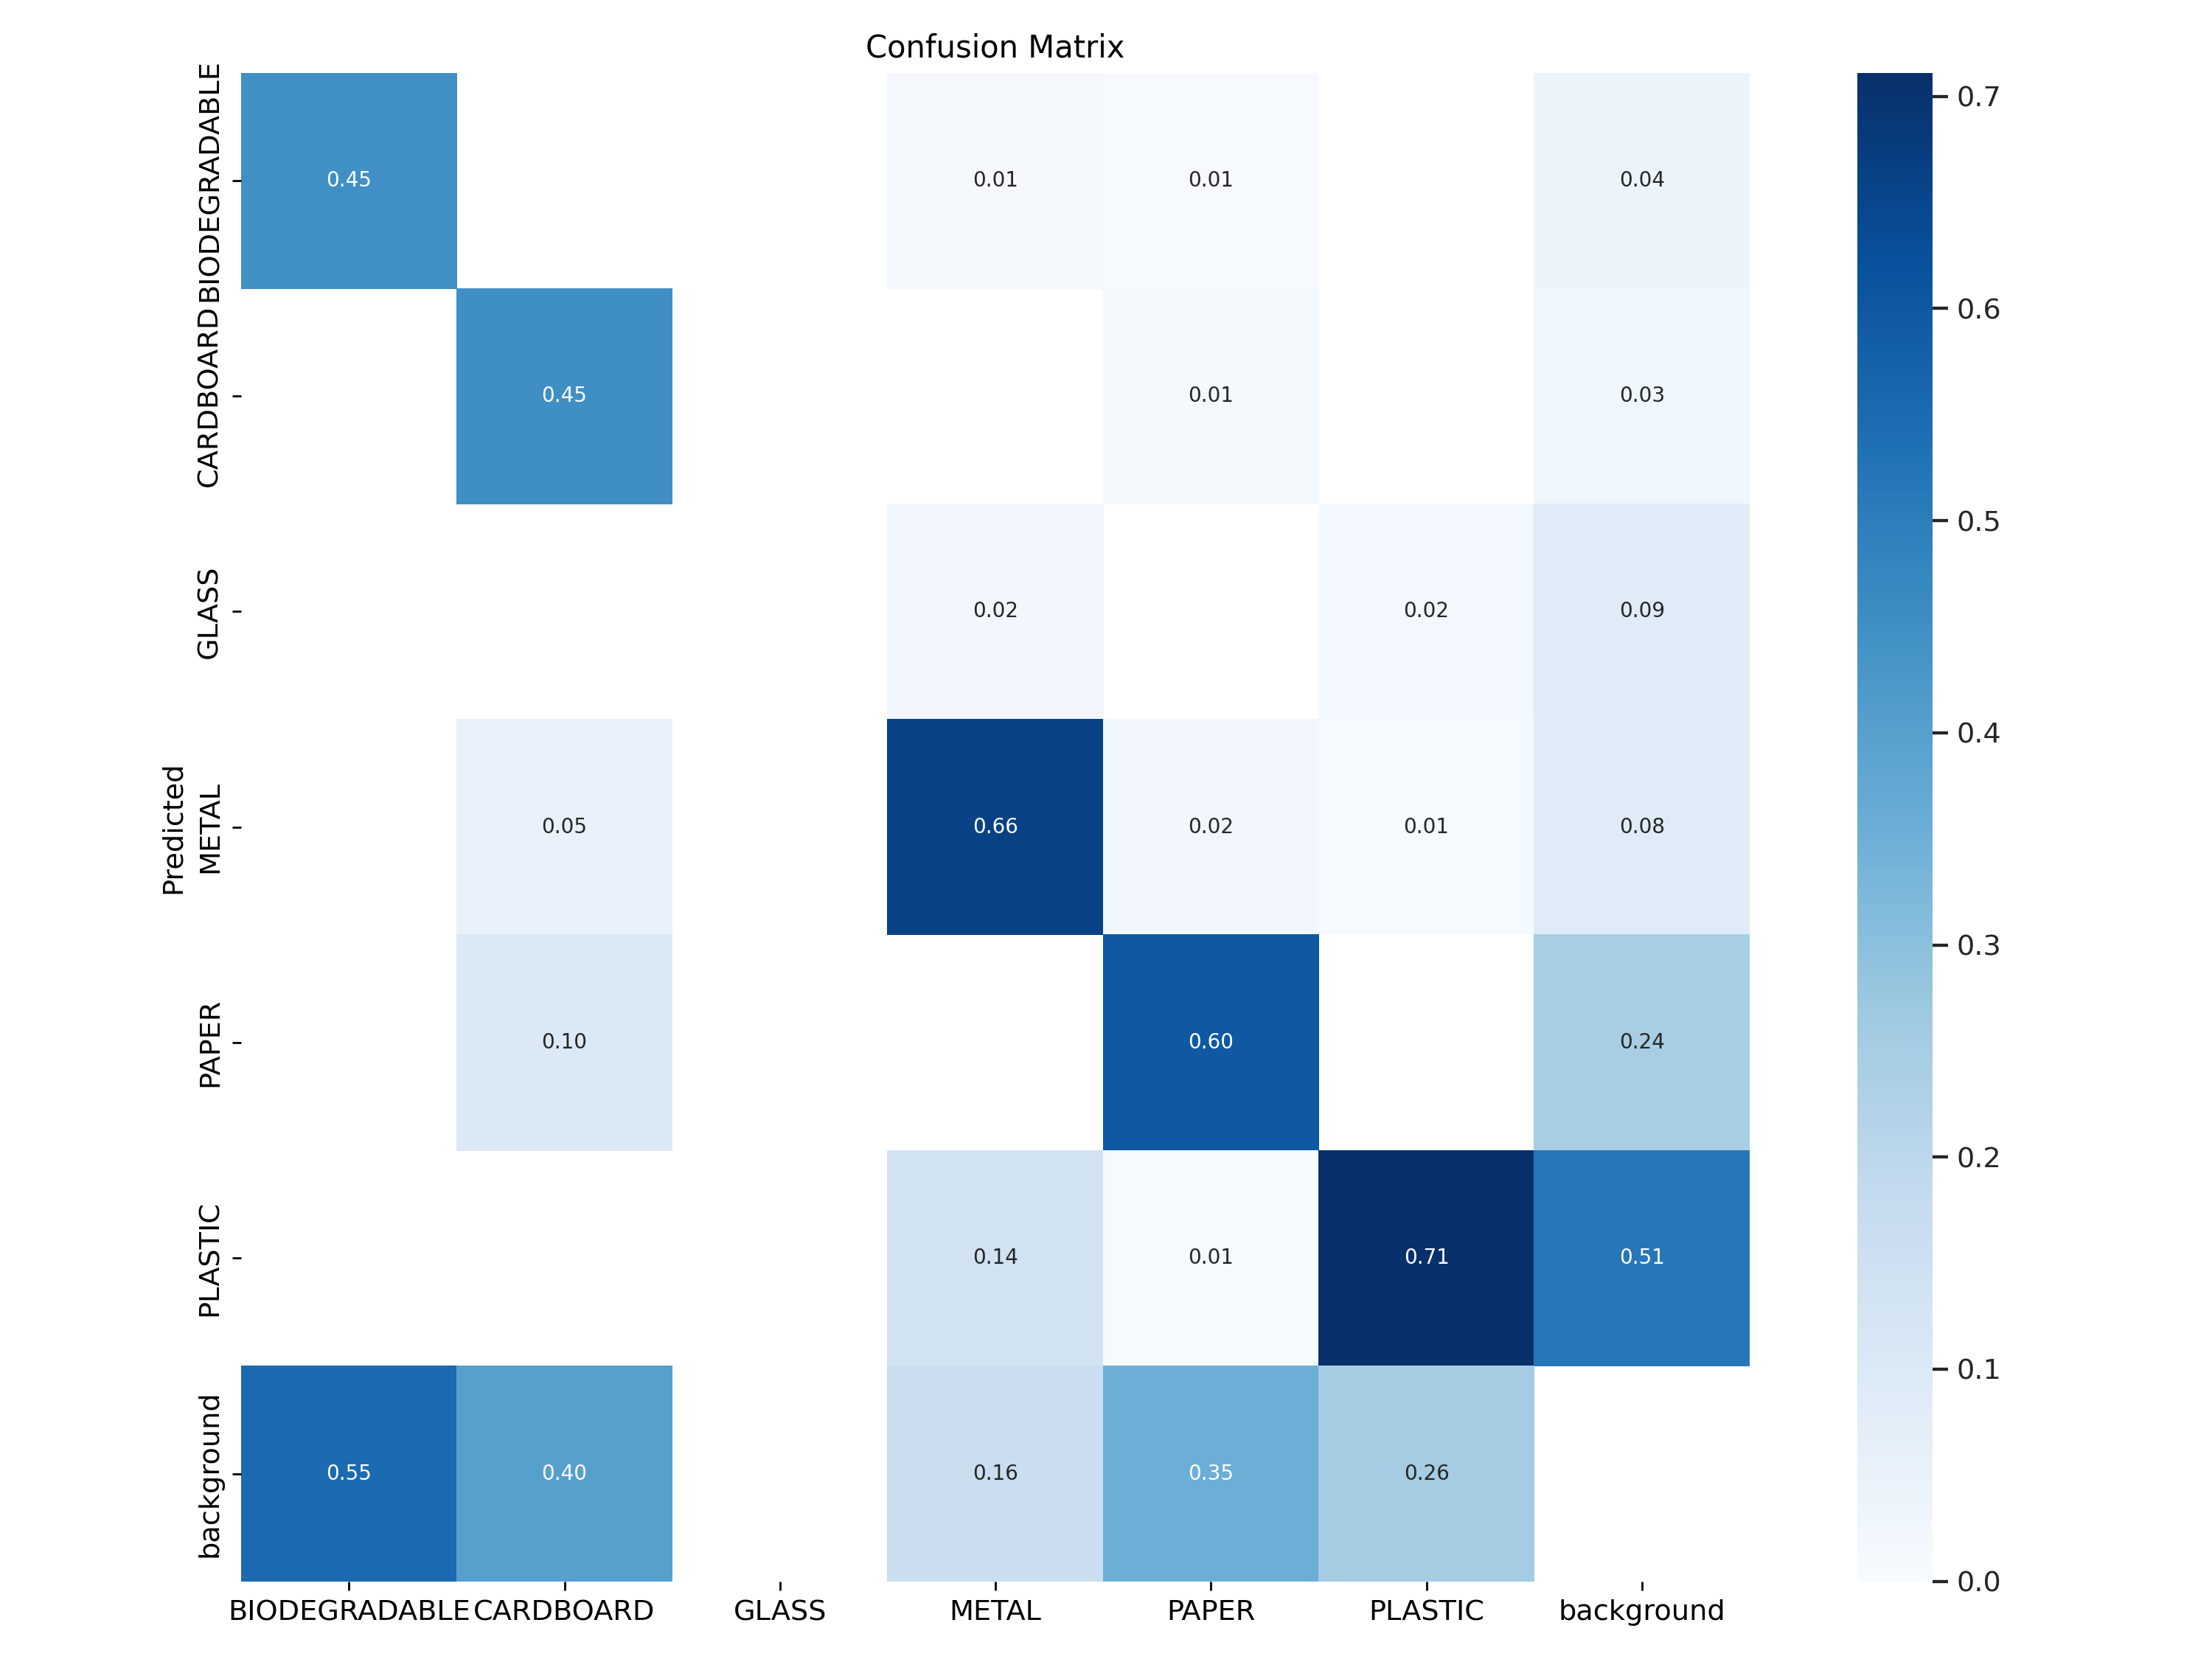
\includegraphics[width=5cm]{Final_Project/image/confusion_matrix.png}
    \caption{Confusion Matrix}
    \label{fig:my_label}
\end{figure}
\\
\\

\bibliography{example_paper}
\bibliographystyle{icml2019}
\clearpage
% Create an appendix in LaTeX

\tableofcontents

\chapter{Github Address}
\\{https://github.com/alsdbtjd0103/COSE474\_Final\_Project.git}

\appendix
\end{document}


